\begin{tikzpicture}[x=.4\marginparwidth,y=.4\marginparwidth,>=stealth]
%\begin{axis}[width=\marginparwidth+25pt,tick label style={font=\scriptsize},axis y line=middle,axis x line=middle,ymin=-1.1,ymax=1.1,xmin=-1.1,xmax=1.1,xtick={1},ytick={1},name=myplot]
%\end{axis}
\draw (0,0) node [shift={(10pt,4pt)}] {\scriptsize$\theta$} circle (1);
\draw [<->] (-1.1,0) -- (1.1,0);
\draw [<->] (0,-1.1) -- (0,1.1);
\draw (0,0) -- (1,.839) node [above] {\scriptsize$(1,\tan \theta)$}-- (1,0) -- (.766,.643);
\fill [black] (1,.839) circle (1.5pt);
\fill [black] (.766,.643) node [left] {\scriptsize$(\cos \theta,\sin \theta)$} circle (1.5pt);
\fill [black] (1,0) node [below right] {\scriptsize$(1,0)$} circle (1.5pt);
\end{tikzpicture}
% this is the sqrt[x] on [0,5]



